\chapter{残余应力和变形}

残余应力和变形计算是多尺度问题,小尺度采用热循环计算,如图\ref{fig:4-1},大尺度采用固有应变法,如图\ref{fig:4-4}。在热循环计算中采用生死单元法,生死单元有两种情况,一种是计算区域是有真实的变化,需要添加网格单元,暂时称为激活单元,如图\ref{fig:4-2},另外一种情况是计算区域没有变化,通过改变材料系数增加单元,暂时称为静单元,我们采用激活单元和静单元的混合形式,逐层增加网格,然后再对每一层修改材料系数,如图\ref{fig:4-4}。计算区域如图\ref{fig:4-5},和图\ref{fig:4-6}中研究类似,具体几何参数可以调整。具体问题可以只计算热传导,或者计算热弹塑性,热弹塑性采用最简单的理想塑性本构。

\begin{figure}[!htbp]
  \centering
  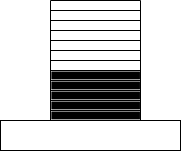
\includegraphics[height=3cm]{fig/4/1.png}
  \caption{热循环残余应力和变形计算}
  \label{fig:4.1.1:1}
\end{figure}

\begin{figure}[!htbp]
  \centering
  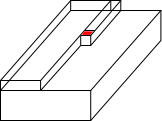
\includegraphics[height=3cm]{fig/4/2.png}
  \caption{激活单元}
  \label{fig:4.1.1:2}
\end{figure}

\begin{figure}[!htbp]
  \centering
  
\includegraphics[height=3cm]{fig/4/3.png}
  \caption{激活单元和静单元混合形式}
  \label{fig:4.1.1:3}
\end{figure}

\begin{figure}[!htbp]
  \centering
  
\includegraphics[height=3cm]{fig/4/4.png}
  \caption{固有应变法残余应力和变形计算}
  \label{fig:4.1.1:4}
\end{figure}

\begin{figure}[!htbp]
  \centering
  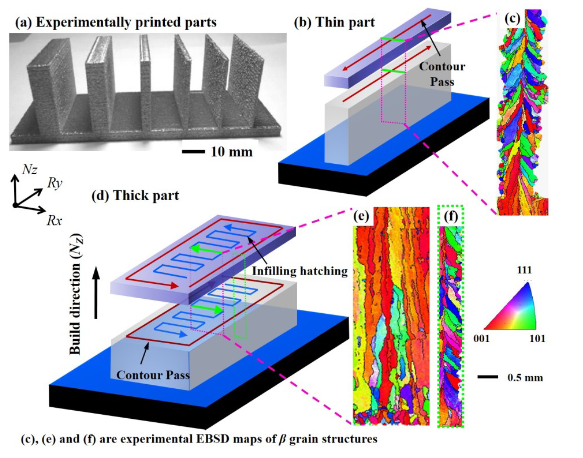
\includegraphics[height=5cm]{fig/4/6.png}
  \caption{固有应变法}
  \label{fig:4.1.1:5}
\end{figure}

\section{热弹塑性}

\subsection{泊松方程}

偏微分方程定义为
\begin{align}\label{eq:4.1.1:1}
  -\Delta u = f \qquad \mathrm{in}\ \Omega\,.
\end{align}

Dirichlet和Neumann边界条件定义为
\begin{subequations}
  \begin{align}\label{eq:4.1.1:2}
    u &= g_{\mathrm D} &\mathrm{on}\ \Gamma_{\mathrm D}\,, \\
    \partial_{\mathbf n}u & = g_{\mathrm N} &\mathrm{on}\ \Gamma_{\mathrm N}\,.
  \end{align}
\end{subequations}

散度定理(Divergence Theorem)为

\begin{align}\label{eq:4.1.1:3}
  \int_{\Omega}\nabla \cdot \mathbf w \ud x = \int_{\Gamma}\mathbf n \cdot \mathbf w \ud s\,.
\end{align}

格林公式(Green's Formula)为

\begin{align}\label{eq:4.1.1:4}
  \int_{\Omega}\mathbf w \cdot \nabla v  \ud x  + \int_{\Omega}\nabla\cdot\mathbf w  v  \ud x = \int_{\Gamma}\mathbf n \cdot \mathbf w v\ud s \,.
\end{align}

如果$\mathbf w=\nabla u$得到

\begin{align}\label{eq:4.1.1:5}
  \int_{\Omega}\nabla u \cdot \nabla v  \ud x  + \int_{\Omega}\nabla\cdot\nabla u  v  \ud x = \int_{\Gamma}\mathbf n \cdot \nabla u v\ud s \,.
\end{align}

方程\eqref{eq:4.1.1:1}两边乘以$v$并做积分得到

\begin{align}\label{eq:4.1.1:6}
  -\int_{\Omega}\Delta uv\ud x &= \int_{\Omega}fv\ud x\,.
\end{align}

将\eqref{eq:4.1.1:5}带入\eqref{eq:4.1.1:6}得到
   
\begin{align}\label{eq:4.1.1:7}
  \int_{\Omega}\nabla u \cdot \nabla v  \ud x = \int_{\Omega}fv\ud x + \int_{\Gamma}\mathbf n \cdot \nabla u v\ud s\,.
\end{align}

根据\eqref{eq:4.1.1:7}定义变分形式。找到$u\in H^1_g$满足

\begin{align}   
  a(u,v)=(f,v) \qquad \forall v\in H^1_0\,.
\end{align}

找到$u_h\in S_{h,g}$满足

\begin{align}   
  a(u_h,\chi)=(f,\chi) \qquad \forall \chi\in S_{h,0}\,.
\end{align}

\begin{align}   
  Ax = b
\end{align}

已知条件如下:
\begin{subequations}
  \begin{align*}
   &u=\mathrm e^{x_1+x_2}\,,\\
   &\Omega:=(0,1)^2\,,\\
   &\Gamma_{\mathrm D}:=\{x|x_1=0\}\bigcup\{x|x_2=0\}\,,\\
   &\Gamma_{\mathrm N}:=\Gamma\setminus\Gamma_{\mathrm D}\,, \\
   &g_{\mathrm D}=\mathrm e^{x_1+x_2}\,,\\
   &g_{\mathrm N}=\mathrm e^{x_1+x_2}\,,\\
    &f=-2\mathrm e^{x_1+x_2}\,.
  \end{align*}
\end{subequations}

表\ref{tab:4.1.1:1}是收敛速度验证,图\ref{fig:4.1.1:1}是level 8的结果图。
\begin{table}[!htbp]\label{tab:4.1.1:1}
  \centering
  \begin{tabular}{c|r|l|l}
    level      &    dof   &         error  &         roc\\
    \hline
    5         &     2113  &         0.00028354  &    3.990265924 \\
    \hline
    6         &     8321  &         7.0922e-05  &    3.9979132 \\
    \hline
    7         &     33025 &         1.7732e-05  &    3.999661629 \\
    \hline
    8         &     131585 &        4.4333e-06  &    3.999729321
  \end{tabular}
  \caption{the Poisson equation, mixed b.c., 2D}
\end{table}

\begin{figure}[!htbp]
  \centering
  
\includegraphics[height=3cm]{fig/4/fig:1.1.1:1.png}
  \caption{the Poisson equation, mixed b.c., 2D}
  \label{fig:4.1.1:1}
\end{figure}

已知条件如下:

\begin{subequations}
  \begin{align*}
   &u=\mathrm e^{x_1+x_2+x_3}\,,\\
   &\Omega:=(0,1)^3\,,\\
   &\Gamma_{\mathrm D}:=\{x|x_1=0\}\bigcup\{x|x_2=0\}\bigcup\{x|x_3=0\}\,,\\
   &\Gamma_{\mathrm N}:=\Gamma\setminus\Gamma_{\mathrm D}\,, \\
   &g_{\mathrm D}=\mathrm e^{x_1+x_2+x_3}\,,\\
   &g_{\mathrm N}=\mathrm e^{x_1+x_2+x_3}\,,\\
    &f=-3\mathrm e^{x_1+x_2+x_3}\,.
  \end{align*}
\end{subequations}


   
表\ref{tab:4.1.1:2}是收敛速度验证,\ref{fig:4.1.1:2}是level 6的结果图。

\begin{table}[!htbp]\label{tab:4.1.1:2}
  \centering
  \begin{tabular}{c|r|l|l}
    level    &      dof   &         error  &         roc \\
    \hline
    3      &        2465  &         0.010258    &    3.776857087 \\
    \hline
    4      &        17985 &         0.0026009  &     3.944019378 \\
    \hline
    5      &        137345   &      0.00065152  &    3.992049361 \\
    \hline
   6      &        1073409   &     0.00016299  &    3.997300448
  \end{tabular}
  \caption{the Poisson equation, mixed b.c., 3D}
\end{table}

\begin{figure}[!htbp]
  \centering
  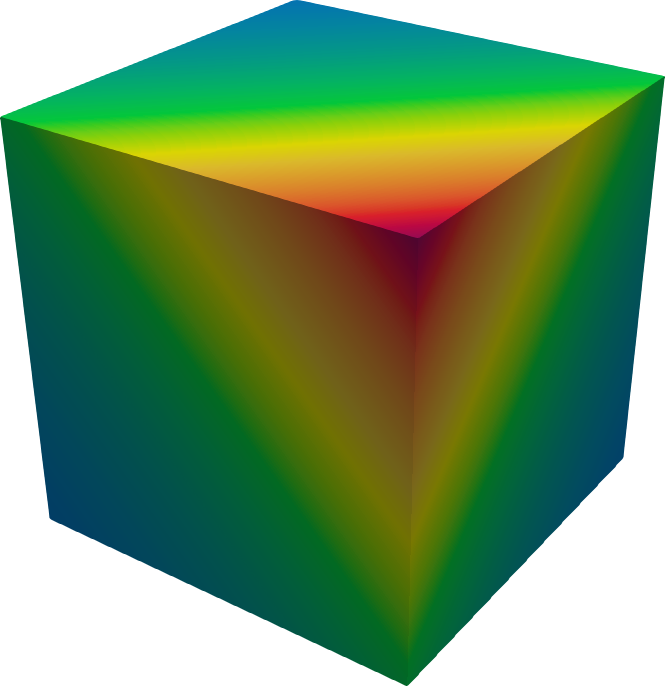
\includegraphics[height=3cm]{fig/4/fig:1.1.1:2.png}
  \caption{the Poisson equation, mixed b.c., 3D}
  \label{fig:4.1.1:2}
\end{figure}

\iffalse
.. _fig-1.1.1-2:

.. figure:: ../../images/fig:1.1.1:2.png
   :alt: Logo
   :align: center
   :height: 130px

   the Poisson equation, mixed b.c., 3D


热传导方程
""""""""""""""""""""

偏微分方程定义为

.. math::
   :label: eq:1.1.2:1

   u_t - \Delta u = f \qquad \mathrm{in}\ \Omega\times\mathrm R_+\,.

Dirichlet和Neumann边界条件定义为
   
.. math::
   :label: eq:1.1.2:2
		   
   u &= g_{\mathrm D} &\mathrm{on}\ \Gamma_{\mathrm D}\times\mathrm R_+\,,
	  
   \partial_{\mathbf n}u & = g_{\mathrm N} &\mathrm{on}\ \Gamma_{\mathrm N}\times\mathrm R_+\,.

初始条件定义为

.. math::
   :label: eq:1.1.2:3
		   
   u(\cdot,0) = v \qquad \mathrm{in}\ \Omega\,.

找到 :math:`u\in H^1_g` 满足

.. math::
   :label: eq:1.1.2:4
   
   (u_t,\varphi) + a(u,\varphi)=(f,\varphi) \qquad \forall \varphi\in H^1_0, t>0\,.

找到 :math:`u_h\in S_{h,g}` 满足

.. math::
   :label: eq:1.1.2:5

   (u_{h,t},\chi) + a(u_h,\chi)=(f,\chi) \qquad \forall \chi\in S_{h,0}, t>0\,.

对时间进行离散

.. math::

   \overline\partial_t U^n = \frac{U^n - U^{n-1}}{k}\,.

找到 :math:`U^n\in S_{h,g}` 满足

.. math::
   :label: eq:1.1.2:6

   \left(\frac{U^n - U^{n-1}}{k},\chi\right) + a(U^n,\chi)=(f^n,\chi) \qquad \forall \chi\in S_{h,0}

.. math::

   \left(U^n,\chi\right) + ka(U^n,\chi)=(kf^n,\chi) + \left(U^{n-1},\chi\right)

.. math::
   :label: eq:1.1.2:7
   
   Ax = b

已知条件如下:

.. math::
   
   &u=\mathrm e^t \mathrm e^{x_1+x_2}\,,\\
   &\Omega:=(0,1)^2\,,\\
   &\Gamma_{\mathrm D}:=\{x|x_1=0\}\bigcup\{x|x_2=0\}\,,\\
   &\Gamma_{\mathrm N}:=\Gamma\setminus\Gamma_{\mathrm D}\,, \\
   &g_{\mathrm D}=\mathrm e^t \mathrm e^{x_1+x_2}\,,\\
   &g_{\mathrm N}=\mathrm e^t \mathrm e^{x_1+x_2}\,,\\
   &f=-\mathrm e^t \mathrm e^{x_1+x_2}\,,\\
   &v=\mathrm e^{x_1+x_2}\,.
   
:numref:`tab:1.1.2:1` 是收敛速度验证, :numref:`fig-1.1.2-1` 是level 8的结果图。

.. table:: the Heat equation, mixed b.c., 2D, :math:`T=0.5`
   :widths: auto
   :name: tab:1.1.2:1

   ============== ============== ==============  ==============
   level          dof            error           roc
   ============== ============== ==============  ==============
	3,7            145           0.007936        3.891003024
    4,9            545           0.0019999       3.96819841
    5,11           2113          0.00050099      3.991896046
    6,13           8321          0.0001253       3.998324022
   ============== ============== ==============  ============== 
   
.. _fig-1.1.2-1:

.. figure:: ../../images/fig:1.1.2:1.png
   :alt: Logo
   :align: center
   :height: 130px

   the Heat equation, mixed b.c., 2D, :math:`T=0.5`

已知条件如下:

.. math::
   
   &u=\mathrm e^t\mathrm e^{x_1+x_2+x_3}\,,\\
   &\Omega:=(0,1)^3\,,\\
   &\Gamma_{\mathrm D}:=\{x|x_1=0\}\bigcup\{x|x_2=0\}\bigcup\{x|x_3=0\}\,,\\
   &\Gamma_{\mathrm N}:=\Gamma\setminus\Gamma_{\mathrm D}\,, \\
   &g_{\mathrm D}=\mathrm e^t\mathrm e^{x_1+x_2+x_3}\,,\\
   &g_{\mathrm N}=\mathrm e^t\mathrm e^{x_1+x_2+x_3}\,,\\
   &f=-2\mathrm e^t\mathrm e^{x_1+x_2+x_3}\,,\\
   &v=\mathrm e^{x_1+x_2+x_3}\,.
   
:numref:`tab:1.1.2:2` 是收敛速度验证, :numref:`fig-1.1.2-2` 是level 6的结果图。

.. table:: the Heat equation, mixed b.c., 3D, :math:`T=0.5`
   :widths: auto
   :name: tab:1.1.2:2

   ============== ============== ==============  ==============
   level          dof            error           roc
   ============== ============== ==============  ==============
	  2,5         369            0.062935
      3,7         2465           0.016651        3.779652874
      4,9         17985          0.0042227       3.943211689
      5,11        137345         0.0010577       3.992341874
   ============== ============== ==============  ============== 

.. _fig-1.1.2-2:

.. figure:: ../../images/fig:1.1.2:2.png
   :alt: Logo
   :align: center
   :height: 130px

   the Heat equation, mixed b.c., 3D, :math:`T=0.5`


热力耦合
""""""""""""""""""""

首先定义热弹性问题。这里需要注意的是方程中 :math:`\mathbf\sigma` 不是全部应力,是去掉温度场影响后的应力。

.. math::
   
  & -\nabla\cdot\mathbf \sigma = \mathbf b \\
  & \rho c\frac{\ud T}{\ud t} + \nabla\cdot \left(\mathbf K \nabla T\right)  = r\\
  & \varepsilon_T = \alpha(T-T_0)\delta_{ij} \\
  &\mathbf\sigma = \mathbf D(\mathbf\varepsilon-\mathbf\varepsilon_T)

.. math::
   
  \mathbf\sigma =& \mathbf D(\mathbf\varepsilon-\mathbf\varepsilon_T)\\
  =&2\mu(\mathbf\varepsilon-\mathbf\varepsilon_T) + \lambda\mathrm{tr}(\mathbf \varepsilon-\mathbf\varepsilon_T)\mathbf 1\\
  =&2\mu\mathbf\varepsilon + \lambda\mathrm{tr}(\mathbf \varepsilon)\mathbf 1 - 2\mu\mathbf\varepsilon_T - \lambda\mathrm{tr}(\mathbf\varepsilon_T)\mathbf 1\\
  =&2\mu\mathbf\varepsilon + \lambda\mathrm{tr}(\mathbf \varepsilon)\mathbf 1 - 2\mu\mathbf\varepsilon_T - \lambda3\alpha (T-T_0)\mathbf 1

.. math::
   
   -\int_{\Omega}\nabla\cdot\mathbf \sigma\cdot\mathbf v\ud x =& \int_{\Omega}\mathbf b\cdot\mathbf v\ud x \\
   -\int_{\Gamma}\mathbf\sigma\cdot\mathbf n\cdot\mathbf v\ud s_x      +\int_{\Omega}\mathbf\sigma:\mathbf\varepsilon(\mathbf v)\ud x =& \int_{\Omega}\mathbf b\cdot\mathbf v\ud x\\
   \int_{\Omega}\left(2\mu\mathbf \varepsilon(\mathbf u) :\mathbf\varepsilon(\mathbf v)+\lambda\nabla\cdot\mathbf u \nabla\cdot\mathbf v\right)\ud x =&
   \int_{\Gamma} \alpha(T-T_0)(3\lambda+2\mu)\mathbf 1:\mathbf\varepsilon(\mathbf v)\ud x + \int_{\Gamma}\mathbf t\cdot\mathbf v\ud s_x + \int_{\Omega}\mathbf b\cdot\mathbf v\ud x

.. math::
   
   \int_{\Omega}(-\nabla\cdot(2\mu\mathbf\varepsilon + \lambda\mathrm{tr}(\mathbf \varepsilon)\mathbf 1))\cdot\mathbf v \ud x
   = \int_{\Omega}\mathbf b\cdot\mathbf v\ud x  + \int_{\Omega} T\nabla\cdot\mathbf v \ud x - \int_{\Gamma}\mathbf n\cdot\mathbf v T\ud s_x 

.. math::
   
  \int_{\Omega}\frac{\ud T}{\ud t}v\ud x - \int_{\Omega}\nabla\cdot \left(\nabla T\right)v\ud x   =& \int_{\Omega}rv\ud x \\
  \int_{\Omega}\frac{\ud T}{\ud t}v\ud x + \int_{\Omega}\nabla T\cdot\nabla v\ud x   =& \int_{\Omega}rv\ud x + \int_{\Gamma}\mathbf n\cdot\nabla T v\ud s_x
  
热应力2D和Abaqus比较,杨氏模量为2.5,泊松比为0.25,热传导为1,比热为1,密度为1,膨胀系数为1,底部固定,上边温度为1,左右下边热流为0,上边方向向上拖拽力为0.1。  

.. _fig-3.4.3-1:

.. figure:: ../../images/3/3.4.3/3.10.5:1.png
   :alt: Logo
   :align: center
   :height: 130px
	    
   :math:`T` ,level 5-6, :math:`\mathrm{time}=0.5` , :math:`T_{max}=0.6247779726982117`

.. _fig-3.4.3-2:

.. figure:: ../../images/3/3.4.3/3.10.5:2.png
   :alt: Logo
   :align: center
   :height: 130px

   :math:`T` ,level 5-6, :math:`\mathrm{time}=0.5` , :math:`\|\mathbf u\|_{max}=1.1456380793904821`

.. _fig-3.4.3-3:

.. figure:: ../../images/3/3.4.3/3.10.5:3.png
   :alt: Logo
   :align: center
   :height: 130px

   :math:`T` , :math:`h=0.025` , :math:`k=0.0125` , :math:`\mathrm{time}=0.5` , :math:`T_{max}=6.221\mathrm e-01`
	   
.. _fig-3.4.3-4:

.. figure:: ../../images/3/3.4.3/3.10.5:4.png
   :alt: Logo
   :align: center
   :height: 130px

   :math:`T` , :math:`h=0.025` , :math:`k=0.0125` , :math:`\mathrm{time}=0.5` , :math:`\|\mathbf u\|_{max}=1.144`

热应力3D和Abaqus比较,杨氏模量为2.5,泊松比为0.25,热传导为1,比热为1,密度为1,膨胀系数为1,底部固定,上边温度为1,左右下边热流为0,上边方向向上拖拽力为0.1。  

.. _fig-3.4.3-5:

.. figure:: ../../images/3/3.4.3/3.10.5:5.png
   :alt: Logo
   :align: center
   :height: 130px
	    
   :math:`T` ,level 0-6, :math:`\mathrm{time}=0.5` , :math:`T_{max}=0.6236979961395264`

.. _fig-3.4.3-6:

.. figure:: ../../images/3/3.4.3/3.10.5:6.png
   :alt: Logo
   :align: center
   :height: 130px

   :math:`T` ,level 5-6, :math:`\mathrm{time}=0.5` , :math:`\|\mathbf u\|_{max}=1.1469914204042906`

.. _fig-3.4.3-7:

.. figure:: ../../images/3/3.4.3/3.10.5:7.png
   :alt: Logo
   :align: center
   :height: 130px

   :math:`T` , :math:`h=0.05` , :math:`k=0.0125` , :math:`\mathrm{time}=0.5` , :math:`T_{max}=6.218\mathrm e-01`
	   
.. _fig-3.4.3-8:

.. figure:: ../../images/3/3.4.3/3.10.5:8.png
   :alt: Logo
   :align: center
   :height: 130px

   :math:`T` , :math:`h=0.05` , :math:`k=0.0125` , :math:`\mathrm{time}=0.5` , :math:`\|\mathbf u\|_{max}=1.144`

其次对于热弹塑性问题,屈服准则受到温度影响,例如理想塑性的屈服准则 :eq:`eq:1.1.2:8` , :math:`\sigma_\theta` 是温度的函数。

.. math::
   :label: eq:1.1.2:8
	   
   f = \mathbf S:\mathbf S-\frac{2}{3}\sigma^2_\theta
\fi
\section{小尺度热循环生死单元法}

\section{构件尺度固有应变法}
